\documentclass[10pt]{article}\usepackage[]{graphicx}\usepackage[]{color}
%% maxwidth is the original width if it is less than linewidth
%% otherwise use linewidth (to make sure the graphics do not exceed the margin)
\makeatletter
\def\maxwidth{ %
  \ifdim\Gin@nat@width>\linewidth
    \linewidth
  \else
    \Gin@nat@width
  \fi
}
\makeatother

\definecolor{fgcolor}{rgb}{0.345, 0.345, 0.345}
\newcommand{\hlnum}[1]{\textcolor[rgb]{0.686,0.059,0.569}{#1}}%
\newcommand{\hlstr}[1]{\textcolor[rgb]{0.192,0.494,0.8}{#1}}%
\newcommand{\hlcom}[1]{\textcolor[rgb]{0.678,0.584,0.686}{\textit{#1}}}%
\newcommand{\hlopt}[1]{\textcolor[rgb]{0,0,0}{#1}}%
\newcommand{\hlstd}[1]{\textcolor[rgb]{0.345,0.345,0.345}{#1}}%
\newcommand{\hlkwa}[1]{\textcolor[rgb]{0.161,0.373,0.58}{\textbf{#1}}}%
\newcommand{\hlkwb}[1]{\textcolor[rgb]{0.69,0.353,0.396}{#1}}%
\newcommand{\hlkwc}[1]{\textcolor[rgb]{0.333,0.667,0.333}{#1}}%
\newcommand{\hlkwd}[1]{\textcolor[rgb]{0.737,0.353,0.396}{\textbf{#1}}}%

\usepackage{framed}
\makeatletter
\newenvironment{kframe}{%
 \def\at@end@of@kframe{}%
 \ifinner\ifhmode%
  \def\at@end@of@kframe{\end{minipage}}%
  \begin{minipage}{\columnwidth}%
 \fi\fi%
 \def\FrameCommand##1{\hskip\@totalleftmargin \hskip-\fboxsep
 \colorbox{shadecolor}{##1}\hskip-\fboxsep
     % There is no \\@totalrightmargin, so:
     \hskip-\linewidth \hskip-\@totalleftmargin \hskip\columnwidth}%
 \MakeFramed {\advance\hsize-\width
   \@totalleftmargin\z@ \linewidth\hsize
   \@setminipage}}%
 {\par\unskip\endMakeFramed%
 \at@end@of@kframe}
\makeatother

\definecolor{shadecolor}{rgb}{.97, .97, .97}
\definecolor{messagecolor}{rgb}{0, 0, 0}
\definecolor{warningcolor}{rgb}{1, 0, 1}
\definecolor{errorcolor}{rgb}{1, 0, 0}
\newenvironment{knitrout}{}{} % an empty environment to be redefined in TeX

\usepackage{alltt}
\usepackage[english]{babel}
\usepackage[utf8]{inputenc}
\usepackage[T1]{fontenc}
\usepackage{indentfirst}
\usepackage{newlfont}
\usepackage{amssymb}
\usepackage{amsmath}
\IfFileExists{upquote.sty}{\usepackage{upquote}}{}
\begin{document}
\author{Giacinto Maggiore}
\title{Simulation of an Exponential random variable}
\maketitle




The goal of the project is to investigate a  $0.2$-exponential distribution in R and the distribution of avarages of $40$ $0.2$-exponentials.We will make  a comparision between the simulated distribution from a sample of 1000 means of 40 exponentials and the theoretical results of CLT.

\section{Theoretical mean  and sample mean}
First of all we construct the sample means.

\begin{knitrout}
\definecolor{shadecolor}{rgb}{0.969, 0.969, 0.969}\color{fgcolor}\begin{kframe}
\begin{alltt}
\hlkwd{set.seed}\hlstd{(}\hlnum{20893}\hlstd{)}
\hlstd{lambda}\hlkwb{<-}\hlnum{.2}
\hlstd{n}\hlkwb{<-}\hlnum{40}
\hlstd{nsim}\hlkwb{<-}\hlnum{1000}
\hlstd{sample}\hlkwb{<-}\hlkwd{matrix}\hlstd{(}\hlkwc{data} \hlstd{=} \hlkwd{rexp}\hlstd{(n}\hlopt{*}\hlstd{nsim,lambda),}\hlkwc{nrow} \hlstd{=} \hlnum{40}\hlstd{,}
               \hlkwc{ncol} \hlstd{=} \hlnum{1000}\hlstd{)}
\hlstd{sampleMeans}\hlkwb{<-}\hlkwd{colMeans}\hlstd{(sample)}
\hlstd{m}\hlkwb{<-}\hlkwd{mean}\hlstd{(sampleMeans)}
\end{alltt}
\end{kframe}
\end{knitrout}

The mean of the sample is 5.021, that is close to the theoretical mean $\frac{1}{\lambda} = 5$. This is underlined in the following plot:
\begin{knitrout}
\definecolor{shadecolor}{rgb}{0.969, 0.969, 0.969}\color{fgcolor}\begin{kframe}
\begin{alltt}
\hlkwd{qplot}\hlstd{(sampleMeans,}
         \hlkwc{main} \hlstd{=} \hlstr{"Histogram for Sample Means"}\hlstd{,}
         \hlkwc{fill}\hlstd{=}\hlkwd{I}\hlstd{(}\hlstr{"lightgrey"}\hlstd{),}
         \hlkwc{col}\hlstd{=}\hlkwd{I}\hlstd{(}\hlstr{"darkgrey"}\hlstd{))}\hlopt{+}
         \hlkwd{xlab}\hlstd{(}\hlstr{"Mean"}\hlstd{)}\hlopt{+}
         \hlkwd{ylab}\hlstd{(}\hlstr{"count"}\hlstd{)}\hlopt{+}
         \hlkwd{geom_vline}\hlstd{(}\hlkwc{xintercept} \hlstd{=} \hlkwd{mean}\hlstd{(sampleMeans),}\hlkwc{col}\hlstd{=}\hlstr{"red"}\hlstd{)}\hlopt{+}
         \hlkwd{geom_vline}\hlstd{(}\hlkwc{xintercept} \hlstd{=} \hlnum{5}\hlstd{,}\hlkwc{col} \hlstd{=} \hlstr{"green"}\hlstd{)}\hlopt{+}
         \hlkwd{theme_minimal}\hlstd{()}
\end{alltt}


{\ttfamily\noindent\itshape\color{messagecolor}{\#\# `stat\_bin()` using `bins = 30`. Pick better value with `binwidth`.}}\end{kframe}

{\centering 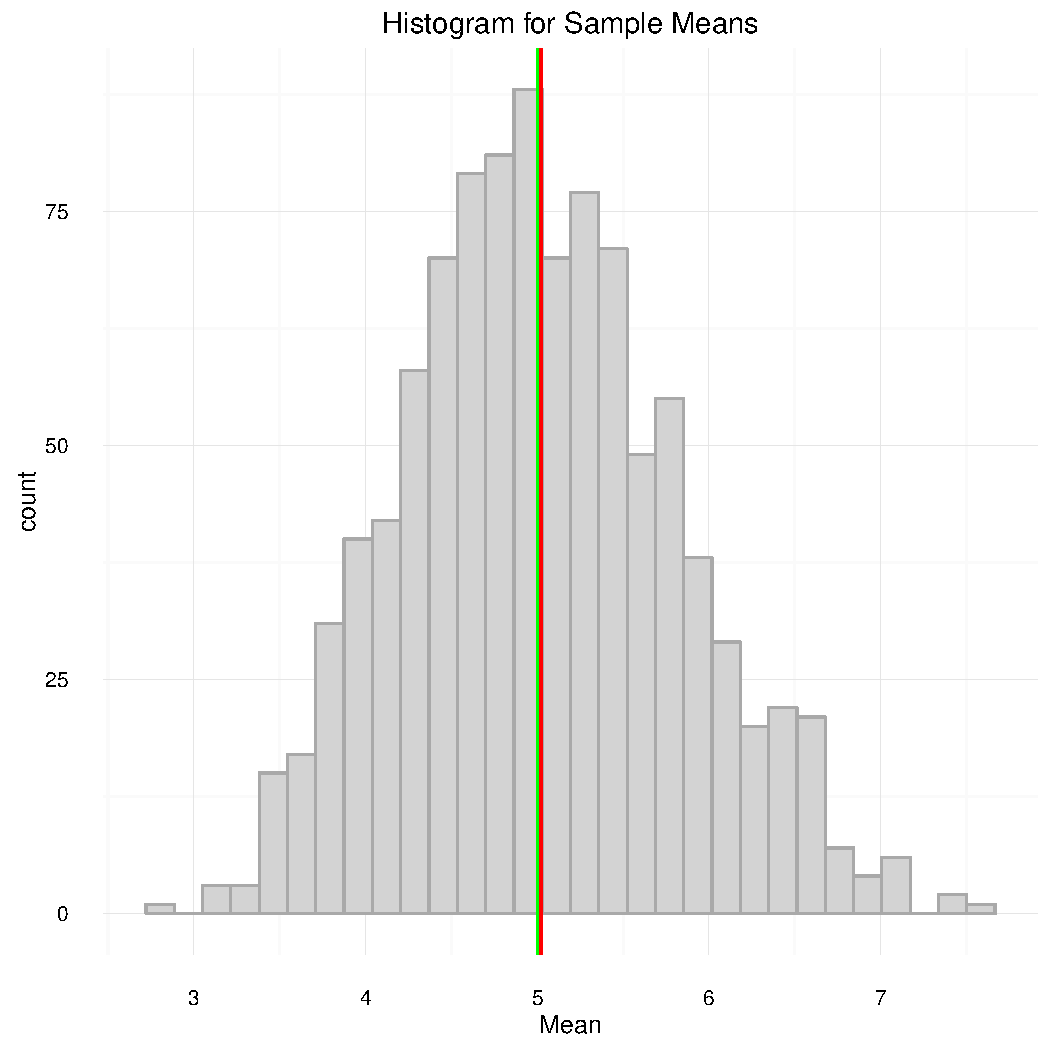
\includegraphics[width=0.6\linewidth]{figure/minimal-mean-plots-1} 

}



\end{knitrout}


\section{Theoretical variance  and sample variance}
In this section we will compare the variance of the sample with the theorical variance of the distribution.

\begin{knitrout}
\definecolor{shadecolor}{rgb}{0.969, 0.969, 0.969}\color{fgcolor}\begin{kframe}
\begin{alltt}
\hlstd{sampleVariance} \hlkwb{<-} \hlstd{(}\hlkwd{sd}\hlstd{(sampleMeans))}\hlopt{^}\hlnum{2}
\hlstd{realVariance} \hlkwb{<-} \hlnum{1}\hlopt{/}\hlstd{((lambda}\hlopt{^}\hlnum{2}\hlstd{)}\hlopt{*}\hlstd{n)}
\end{alltt}
\end{kframe}
\end{knitrout}

The sample variance is 0.629
and the theoretical one is 0.625, so they are  very close.

\section{Distribution of the sample}
\begin{knitrout}
\definecolor{shadecolor}{rgb}{0.969, 0.969, 0.969}\color{fgcolor}\begin{kframe}
\begin{alltt}
\hlstd{x} \hlkwb{<-} \hlkwd{seq}\hlstd{(}\hlnum{2}\hlstd{,}\hlnum{8}\hlstd{,}\hlkwc{by}\hlstd{=}\hlnum{0.1}\hlstd{)}

\hlstd{g}\hlkwb{<-}\hlkwd{ggplot}\hlstd{()} \hlopt{+}
\hlkwd{geom_histogram}\hlstd{(}\hlkwd{aes}\hlstd{(}\hlkwc{x}\hlstd{=sampleMeans,}\hlkwc{y}\hlstd{=..density..),}
              \hlkwc{position}\hlstd{=}\hlstr{"identity"}\hlstd{,}\hlkwc{fill}\hlstd{=}\hlkwd{I}\hlstd{(}\hlstr{"lightgrey"}\hlstd{),}
              \hlkwc{col} \hlstd{= (}\hlstr{"darkgrey"}\hlstd{))}\hlopt{+}
\hlkwd{geom_density}\hlstd{(}\hlkwd{aes}\hlstd{(}\hlkwc{x}\hlstd{=sampleMeans,}\hlkwc{y}\hlstd{=..density..))}\hlopt{+}
\hlkwd{ggtitle}\hlstd{(}\hlstr{"Density of the sample of the means"}\hlstd{)}\hlopt{+}
\hlkwd{xlab}\hlstd{(}\hlstr{"Mean"}\hlstd{)}\hlopt{+}
\hlkwd{geom_line}\hlstd{(}\hlkwd{aes}\hlstd{(}\hlkwc{x}\hlstd{=x,}
        \hlkwc{y}\hlstd{=}\hlkwd{dnorm}\hlstd{(x,}
                \hlkwc{mean} \hlstd{=} \hlnum{1}\hlopt{/}\hlstd{lambda,}
                \hlkwc{sd} \hlstd{=} \hlnum{1}\hlopt{/}\hlstd{(lambda}\hlopt{*}\hlkwd{sqrt}\hlstd{(}\hlnum{40}\hlstd{)))),}
         \hlkwc{color}\hlstd{=}\hlstr{"red"}\hlstd{)}\hlopt{+}
\hlkwd{geom_vline}\hlstd{(}\hlkwc{xintercept} \hlstd{=} \hlnum{5}\hlstd{,}\hlkwc{col} \hlstd{=} \hlstr{"red"}\hlstd{)}

\hlstd{sample}\hlkwb{<-}\hlkwd{rexp}\hlstd{(nsim,lambda)}
\hlstd{p}\hlkwb{<-}\hlkwd{ggplot}\hlstd{()}\hlopt{+}
    \hlkwd{geom_histogram}\hlstd{(}\hlkwd{aes}\hlstd{(}\hlkwc{x}\hlstd{=sample,}\hlkwc{y}\hlstd{=..density..),}
              \hlkwc{position}\hlstd{=}\hlstr{"identity"}\hlstd{,}\hlkwc{fill}\hlstd{=}\hlkwd{I}\hlstd{(}\hlstr{"lightgrey"}\hlstd{),}
              \hlkwc{col} \hlstd{= (}\hlstr{"darkgrey"}\hlstd{))}\hlopt{+}
    \hlkwd{geom_density}\hlstd{(}\hlkwd{aes}\hlstd{(}\hlkwc{x}\hlstd{=sample,}\hlkwc{y}\hlstd{=..density..))}\hlopt{+}
    \hlkwd{ggtitle}\hlstd{(}\hlstr{"Density of a sample of exponential r.v. "}\hlstd{)}\hlopt{+}
    \hlkwd{xlab}\hlstd{(}\hlstr{"Value"}\hlstd{)}\hlopt{+}
    \hlkwd{theme_minimal}\hlstd{()}
\hlkwd{grid.arrange}\hlstd{(g,p)}
\end{alltt}


{\ttfamily\noindent\itshape\color{messagecolor}{\#\# `stat\_bin()` using `bins = 30`. Pick better value with `binwidth`.\\\#\# `stat\_bin()` using `bins = 30`. Pick better value with `binwidth`.}}\end{kframe}

{\centering 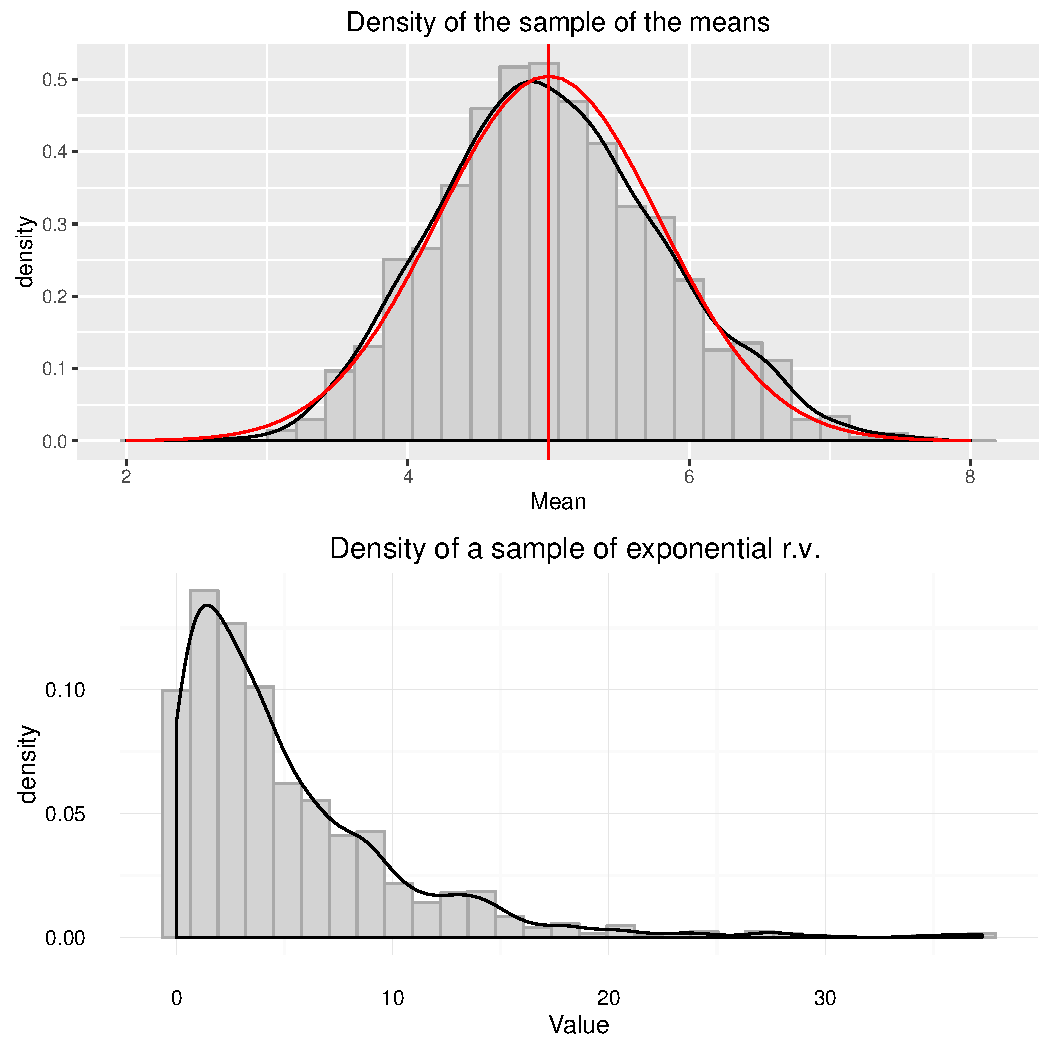
\includegraphics[width=0.7\linewidth]{figure/minimal-distribution-1} 

}



\end{knitrout}

In the first plot the black line represents the simulated distribution density and it is very close to the  normal distribution density (represented by red line) predicted by  Central Limit Theorem. Observe that  there is a lot of difference between the distribution of a large collection of averages of 40 exponentials and the distribution of a large collection of random exponentials. In fact if the first one is approximately normal, the second one has an exponential density, as can be seen in the second plot.  

\end{document}
